\begin{figure}[htbp]
\centering
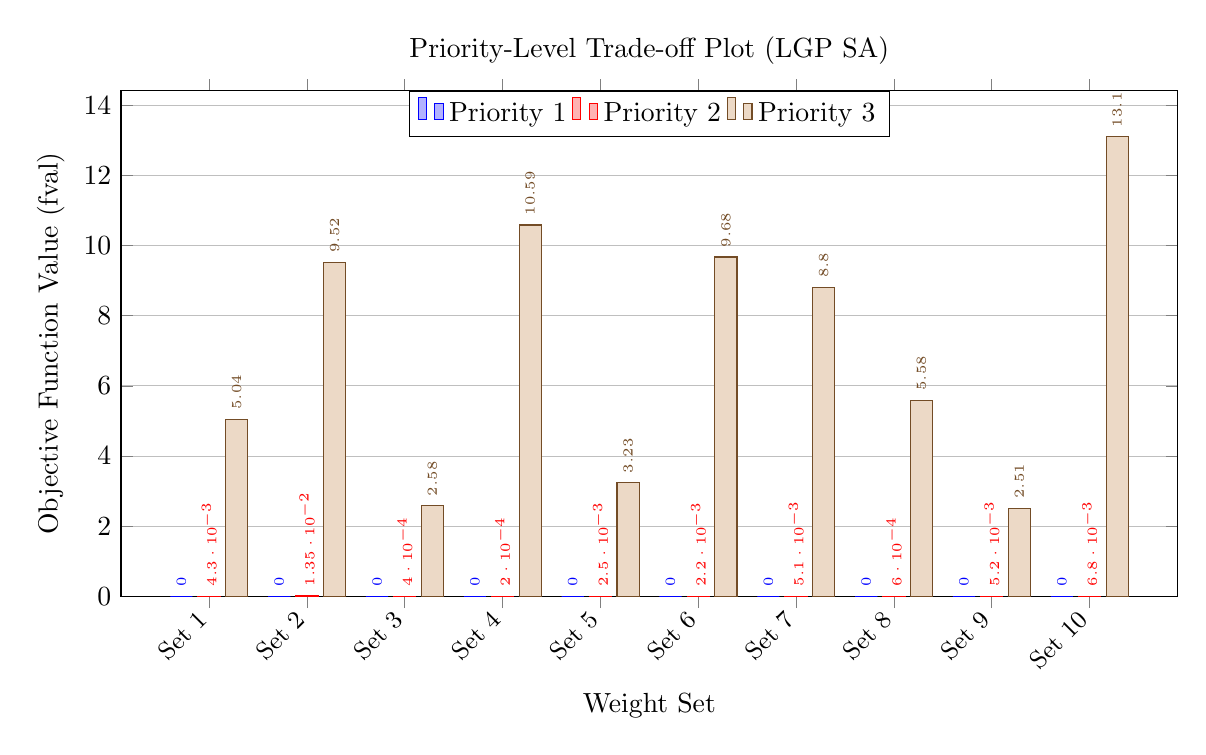
\begin{tikzpicture}
  \begin{axis}[
    ybar,
    bar width=8pt,
    title={Priority-Level Trade-off Plot (LGP SA)},
    xlabel={Weight Set},
    ylabel={Objective Function Value (fval)},
    symbolic x coords={Set 1,Set 2,Set 3,Set 4,Set 5,Set 6,Set 7,Set 8,Set 9,Set 10},
    xtick=data,
    xticklabel style={rotate=45,anchor=east,font=\small},
    width=15cm,
    height=8cm,
    ymin=0,
    enlarge x limits=0.1,
    legend style={at={(0.5,1)},anchor=north,legend columns=3},
    ymajorgrids,
    nodes near coords,
    nodes near coords align={vertical},
    every node near coord/.append style={font=\tiny, rotate=90, anchor=west}
  ]

  % Priority 1 (all zeros)
  \legend{Priority 1, Priority 2, Priority 3}
  \addplot coordinates {(Set 1,0) (Set 2,0) (Set 3,0) (Set 4,0) (Set 5,0) 
                        (Set 6,0) (Set 7,0) (Set 8,0) (Set 9,0) (Set 10,0)};
  % Priority 2
  \addplot coordinates {(Set 1,0.0043) (Set 2,0.0135) (Set 3,0.0004) (Set 4,0.0002) (Set 5,0.0025)
                        (Set 6,0.0022) (Set 7,0.0051) (Set 8,0.0006) (Set 9,0.0052) (Set 10,0.0068)};
  % Priority 3
  \addplot coordinates {(Set 1,5.0425) (Set 2,9.5191) (Set 3,2.5808) (Set 4,10.5879) (Set 5,3.2344)
                        (Set 6,9.6772) (Set 7,8.8018) (Set 8,5.5848) (Set 9,2.5091) (Set 10,13.1004)};

  \end{axis}
\end{tikzpicture}
\caption{Comparison of objective values (\textit{fval}) at Priority 1, 2, and 3 across weight sets for Lexicographic Goal Programming sensitivity analysis. Numbers above bars show exact values.}
\label{fig:lgp_fval_tradeoff}
\end{figure}
